% Sources (checked by shahid.check_numbers): results/cp7_heldout.json results/iforest.json
% results/leak_audit.json results/cp12.json results/p2/confirm.json; ledger C7-01, AU-01, CP12-T5, P2C-01..05, CAD-1..4, TN-H1..H4
\section{Results}\label{sec:results}
All results are SIMULATED.

\subsection{Held-out network and baselines}\label{sec:heldout}
Table~\ref{tab:heldout} compares methods on identical observed inputs: 109 outages and 155
communication failures on the held-out network, test weeks, evaluated once.

\begin{table*}[!t]
\caption{Held-out urban network, test weeks, evaluated once}\label{tab:heldout}
\centering\tabfont
\begin{tabularx}{\textwidth}{@{}L{0.25\textwidth}ZZZZZZZ@{}}
\toprule
\textbf{Method} & \textbf{Coverage} & \textbf{Accuracy when deciding} & \textbf{Outage recall} & \textbf{Comms recall} & \textbf{False outage} & \textbf{Missed outage} & \textbf{Fault-free false outages per meter-day} \\
\midrule
SHAHID version 1 (with abstention) & 0.723 & 0.995 & 0.670 & 0.755 & 0.000 & 0.009 & 0.0010 \\
Two-sided z-test$^{a}$ & 0.636 & 0.994 & 0.615 & 0.645 & 0.000 & 0.009 & 0.0002 \\
Likelihood ratio without abstention$^{a}$ & 0.720 & 0.963 & 0.716 & 0.677 & 0.039 & 0.009 & 0.0038 \\
Visible-share test$^{a}$ & 0.720 & 0.963 & 0.725 & 0.671 & 0.045 & 0.000 & 0.0045 \\
Naive share baseline$^{b}$ & 0.871 & 0.943 & 0.890 & 0.774 & 0.065 & 0.028 & 0.0104 \\
Step baseline (transformer drop) & 1.000 & 0.682 & 0.752 & 0.632 & 0.368 & 0.248 & 0.0629 \\
Count baseline (share of section silent) & 1.000 & 0.545 & 0.826 & 0.348 & 0.652 & 0.174 & 0.0039 \\
Structure baseline (silence pattern)$^{b}$ & 0.765 & 0.604 & 0.624 & 0.348 & 0.394 & 0.174 & 0.0031 \\
Isolation Forest \cite{liu2008isolation} (added afterwards) & 1.000 & 0.447 & 0.972 & 0.077 & 0.923 & 0.028 & 0.0057 \\
\bottomrule
\multicolumn{8}{@{}p{\textwidth}@{}}{\scriptsize $^{a}$Coverage below 1 without an abstention band: these methods answer UNCERTAIN when the expected energy of the silent group is below a minimum chosen on validation weeks; the z-test also when both or neither cause fits. $^{b}$The naive baseline has its own minimum-energy rule; the structure baseline abstains when the silent set is both a concentrator group and a line section. The count and step baselines and the Isolation Forest never abstain.}
\end{tabularx}
\end{table*}

Version 1 is the safest method, not the one that decides most often: the naive baseline decides
0.871 of events but calls 0.065 of communication failures outages. On development validation data,
only version 1 (coverage 0.663) and the z-test (0.602) can meet the three safety limits at any
setting. The Isolation Forest detects that something happened but cannot attribute the cause (AUC
0.41, 95\% interval 0.341--0.484, where AUC is the area under the receiver operating characteristic curve).
\textbf{Leak check:} replacing the transformer series with a copy shifted by seven days drops outage
recall from 0.641 to 0.103; the decisions depend on the transformer signal.

\subsection{Every frozen evaluation}\label{sec:allgrids}
Table~\ref{tab:allgrids} lists every evaluation of the frozen method. The development row uses unseen
weeks of the network on which thresholds were chosen, so it is not held-out data.

\begin{table}[!t]
\caption{Every evaluation of frozen version 1 (95\% Wilson intervals where computed)}\label{tab:allgrids}
\centering\scriptsize\setlength{\tabcolsep}{2pt}
\begin{tabularx}{\columnwidth}{@{}Y C{0.21\columnwidth} C{0.21\columnwidth} C{0.21\columnwidth}@{}}
\toprule
\textbf{Network (run)} & \textbf{Coverage} & \textbf{False outage} & \textbf{Missed outage} \\
\midrule
Development, test weeks & 0.697 (0.639--0.749) & 0.000 (0.000--0.024) & 0.000 (0.000--0.035) \\
Held-out urban (once) & 0.723 (0.667--0.774) & 0.000 (0.000--0.024) & 0.009 (0.002--0.050) \\
Untouched rural (once) & 0.494 (0.421--0.568) & 0.000 (0.000--0.034) & 0.000 (0.000--0.055) \\
Never used, rural, 99 meters (once) & 0.670 (---)$^{a}$ & 0.000 (---)$^{a}$ & 0.009 (---)$^{a}$ \\
Never used, semi-urban, 41 meters (once) & 0.527 (---)$^{a}$ & 0.000 (---)$^{a}$ & 0.000 (---)$^{a}$ \\
\bottomrule
\multicolumn{4}{@{}p{\columnwidth}@{}}{\scriptsize $^{a}$Wilson interval not computed for the confirmatory runs.}
\end{tabularx}
\end{table}

Accuracy when deciding was 1.0 on both never-used networks. The false-outage rates of
Table~\ref{tab:allgrids} (0.000) concern labelled communication failures. On fault-free data the two
never-used networks gave 0.0004 and 0.0006 false outages per meter-day. On data with no events,
random single-meter data losses still produced about 15 to 33 false outage verdicts per
transformer-year under the registered configuration; a post-hoc gate reduced this to 0.2 to 1.0
(Section~\ref{sec:governance}). Across the first three evaluations, outage recall was 0.42--0.67 and
communication recall 0.54--0.75. The median decision latency is 2 intervals after the meters go
silent.

\subsection{Resolution limit and where the method weakens}\label{sec:weakens}
The method is correct with probability 0.90 once the expected silent energy is about 6 times its
predictive uncertainty: a signal-to-noise ratio (SNR) of 6.1 (5.2--7.3) on the development network
and 4.9 (4.2--5.6) on the held-out network (Fig.~\ref{fig:snr}). A single silent customer is below
this limit, so it usually receives an abstention; the rare wrong verdicts on one- and two-meter groups
are the fault-free false outages of Section~\ref{sec:governance}.

\begin{figure}[!t]
\centering
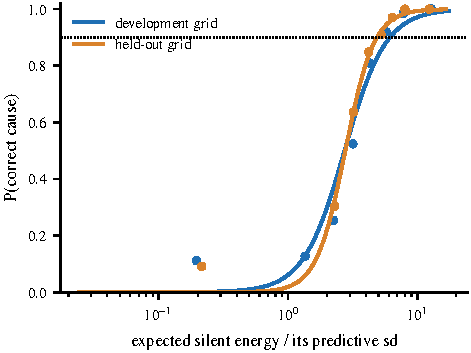
\includegraphics[width=\columnwidth]{figures/snr_detectability.pdf}
\caption{Probability of a correct verdict against the ratio of expected silent energy to its
uncertainty (SIMULATED; dots are binned shares, lines are logistic fits; dotted line at
0.9).}\label{fig:snr}
\end{figure}

Table~\ref{tab:weakens} lists the conditions that degrade the method, on the development network with
frozen thresholds, and the reporting-interval sensitivity on three networks with new seeds
(post-hoc).

\begin{table}[!t]
\caption{Conditions under which version 1 weakens or fails}\label{tab:weakens}
\centering\scriptsize\setlength{\tabcolsep}{2.5pt}
\begin{tabularx}{\columnwidth}{@{}Y C{0.14\columnwidth} C{0.14\columnwidth} C{0.14\columnwidth}@{}}
\toprule
\textbf{Condition} & \textbf{Coverage} & \textbf{False outage} & \textbf{Missed outage} \\
\midrule
Transformer-meter gain error, sd 2\% & 0.567 & 0.019 & 0.046 \\
Load-shaped unmetered energy, 5 kW & 0.534 & 0.034 & 0.122 \\
Load-shaped unmetered energy, 10 kW & 0.538 & 0.045 & 0.241 \\
Outage and communication failure at once & 0.761 & 0.016 & 0.373 \\
10\% of readings lost at random & 0.490 & 0.000 & 0.135 \\
Midday with doubled PV & 0.528 & 0.000 & 0.013 \\
\midrule
Readings every 15 min (three networks) & 0.629 & 0.002 & 0.006 \\
Readings every 30 min & 0.555 & 0.012 & 0.036 \\
Readings every 60 min & 0.421 & 0.021 & 0.245 \\
\bottomrule
\end{tabularx}
\end{table}

\begin{itemize}
\item \textbf{Main weakness.} The method treats the normal gap as constant; unmetered energy that
follows the load and transformer-meter gain error both scale with load (Fig.~\ref{fig:unmetered}).
\item \textbf{Simultaneous events} merge into one silent group that looks like a communication failure.
\item \textbf{Reporting interval.} Quarter-hour readings are safe; half-hour readings are
inconclusive (missed outages 0.036, upper bound 0.052); hourly readings are outside the envelope,
mostly because short events no longer suppress two readings.
\item \textbf{Not sensitive to} constant unmetered energy, meter noise up to three times nominal,
history length, PV share or concentrator layout. Coverage spans 0.484 to 0.663 over the range of the
uncalibrated diversity parameter.
\end{itemize}

\begin{figure}[!t]
\centering
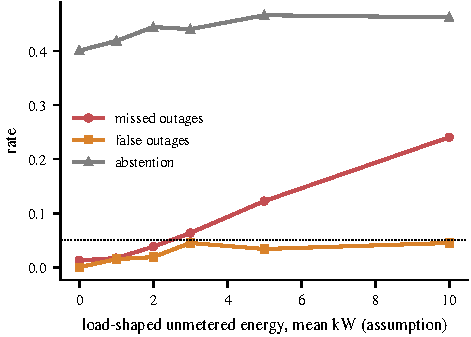
\includegraphics[width=\columnwidth]{figures/unmetered_failure.pdf}
\caption{Missed and false outages, and abstention, as load-shaped unmetered energy increases
(SIMULATED, development network; dotted line at the 5\% limit).}\label{fig:unmetered}
\end{figure}

\subsection{Further studies (protocols committed before running)}\label{sec:phase2}
\begin{itemize}
\item \textbf{Merged powered meter.} A powered meter that goes silent at the same moment as an outage
can join the outage group and supply its residual; on whole-feeder runs of the never-used rural network this happens
15.0 times per transformer-year. This is a different quantity from the 15.0 false outage verdicts
of Section~\ref{sec:governance}: both count 30 events over the same exposure, but in separate
simulations (whole-feeder outages here, fault-free data there). Splitting silent groups by feeder removed every confident wrong verdict it
caused (4 to 0) and stayed within the safety limits, at a price: abstention on random-meter
communication failures rose from 0.405 to 0.973.
\item \textbf{Negative results.} A prior that depends on group size missed 0.107 to 0.321 of
outages, above the limit; evidence accounting version 2 missed more mid-interval outages than version 1
(0.257 against 0.117). Version 1 stays the registered method.
\end{itemize}

\subsection{Deployment modes (Tunisia study)}\label{sec:tunisia}
A further study, on the same simulated networks with new seeds, varied the unknown Tunisian deployment
conditions; every value is an ASSUMPTION. Frozen version 1 transferred in 15 of 24 families and failed
under 10\% random loss and load-shaped unmetered energy. A transformer series delayed by a day costs
only time. Without a transformer measurement, every energy-balance method answers UNSUPPORTED for
0.997 of episodes: the transformer meter is a prerequisite, not an option. With daily batch delivery
the diagnosis becomes retrospective (median delay 10.25 h).
